\documentclass[12pt]{article}
\usepackage{array}
\usepackage{amsmath}
\usepackage{mathtools}
\usepackage{gensymb}
\usepackage{graphicx}
\usepackage{float}
\usepackage{caption}

\allowdisplaybreaks

\begin{document}
    \title{Hooke's Law and Conservation of Energy}
    \author{Ryan Coyne and Patrick Browning}
    \maketitle
    \section{Abstract/Conclusion}
        The spring constant of a spring was measured to be \(3.010 \pm 0.023\) N/m using a force sensor and a motion sensor. The total mechanical energy appeared to be conserved. The mass hung from the spring was marked as fifty grams which was the value that was initially used to calculate the kinetic and gravitational potentially energies. However it was noticed that using forty eight grams in the calculation significantly smoothed the graph of total mechanical energy and when the mass was measured it was found to be forty eight grams.
    \section{Procedure}
        A metal rod was clamped vertically to the edge of a table and a second metal rod was clapped at a ninety degree angle to the first so that it's end was past the edge of the table. A force sensor was attached to the second rod so that it's hook was downward. A spring was hung from the hook. A sonic motion sensor was place on the floor under the spring so that the center of the spring was in line with the center of the motion sensor. The force sensor was zeroed at this time. A weighted metal hanger was held with it's hook in the lowest ring of the spring but without stretching the spring and the motion sensor was zeroed. The hanger was then allowed to hang from the spring and come to rest at equilibrium. Next the hanger was raised approximately two centimeter and allowed to fall and oscillate on the spring. Just after it began to fall the recording for the force and position sensors was started. After about seven cycles, the recording was stopped.
    \section{Data}
        The mass, \(m\), used to find the spring constant and to analyze conservation of energy was 0.048 kg. The spring constant, \(k\), was 3.010 N/m.
        \begin{figure}[H]
            \centering
            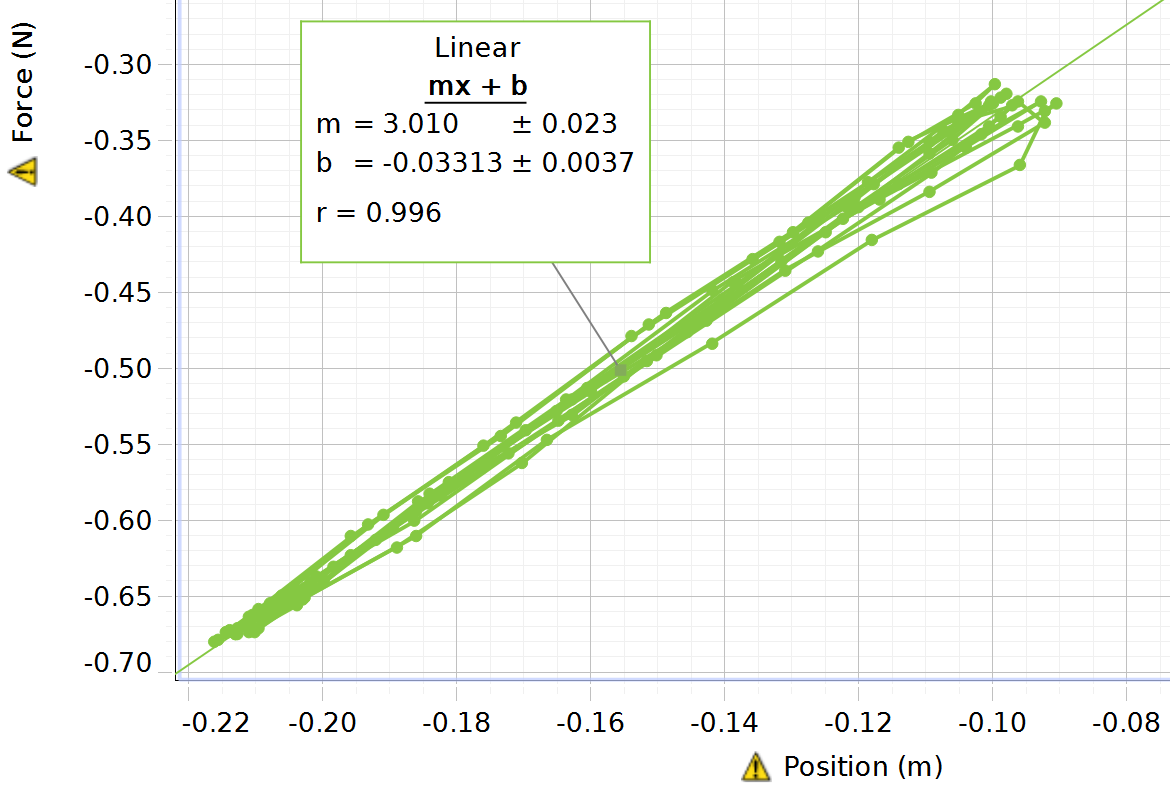
\includegraphics[width=0.78\linewidth]{fx.png}
            \caption{Plot of force vs displacement from equilibrium.}
        \end{figure}
        \begin{figure}[H]
            \centering
            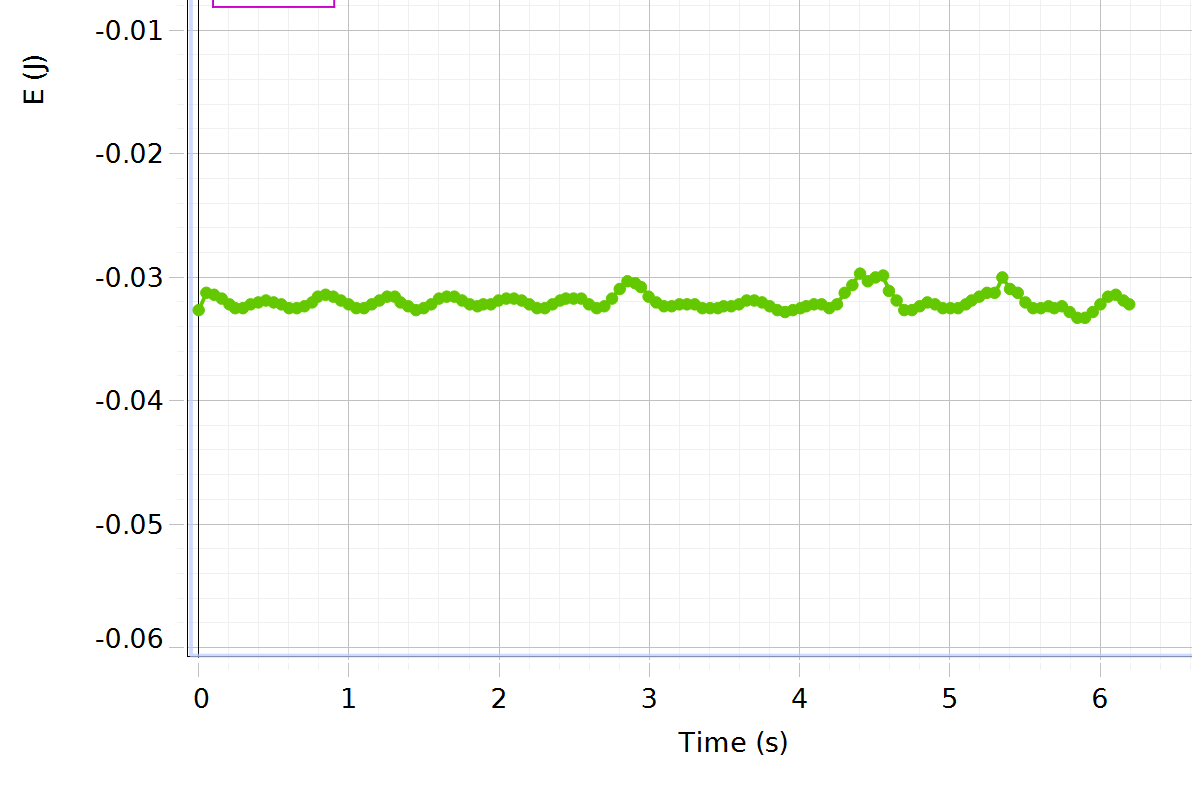
\includegraphics[width=0.78\linewidth]{et.png}
            \caption{Plot of mechanical energy vs time.}
        \end{figure}
\end{document}